\newpage
\section[Day 1: Ordered Sets \& Fields]{ Ordered Sets and Fields }

\subsection{ Ordered Sets and Bounds }

	\begin{definition}{Ordered Set}{14cm}
		An order is:

		\begin{itemize}[leftmargin=1cm, itemsep=0.1cm]
			\item { \color{lblue} Trichotomy}:
				For all x,y $ \in $ S, only one holds true:

				\begin{itemize}[leftmargin=1cm, itemsep=0.1cm]
					\item x $<$ y
					\item x = y
					\item x $>$ y
				\end{itemize}

			\item { \color{lblue} Transitivity}:
				If x $<$ y and y $<$ z, then x $<$ z.
		\end{itemize}

		An ordered set is a set with an order.
	\end{definition}	

	\vspace{0.5cm}



	\begin{definition}{Bounds}{14cm}
		Let S be an ordered set and E $ \subset $ S.

		An upper bound of E is a $ \beta \in $ S such that for x $ \leq \beta $
		for all x $ \in $ E.

		\hspace{1cm}
		If such a $ \beta $ exists, then E is bounded from above.

		A lower bound of E is a $\alpha$ $\in$ S such that for x $ \geq $ $\alpha$
		for all x $\in$ E.

		\hspace{1cm}
		If such a $\alpha$ exists, then E is bounded from below.	
	\end{definition}

	\vspace{0.5cm}



	\begin{definition}{Infimum \& Supremum}{14cm}
		Let S be an ordered set.

		Let E $ \subset $ S be bounded from above.
		Least upper bound $\beta$ $\in$ S exists if:
		
		\begin{itemize}[leftmargin=1.5cm, itemsep=0.1cm]
			\item $\beta$ is an upper bound for E
		
			\item If $\gamma < \beta$, then $ \gamma $ is not an upper bound for E.
		\end{itemize}

		Then $\beta$ = sup(E).

		\vspace{0.3cm}

		Let E $\subset$ S be bounded from below.
		Greatest lower bound $\alpha$ $\in$ S exists if:
		
		\begin{itemize}[leftmargin=1.5cm , itemsep=0.1cm]
			\item $\alpha$ is a lower bound for E

			\item If $\gamma > \alpha$, then $\gamma$ is not a lower bound for E.
		\end{itemize}

		Then $\alpha$ = inf(E).

		\vspace{0.3cm}

		Even if sup(E) exists, it may or may not exists at S.

		If sup(E) exists, then sup(E) is unique.
		Statement also holds true for inf(E).
	\end{definition}
	
	\vspace{0.5cm}



	\begin{example}
		Let S = $ (1,2) \cup [3,4) \cup (5,6) $ with the
		order $ < $ from $ \mathbb{R} $. For subsets E of S:

		\begin{itemize}[leftmargin=1.5cm, itemsep=0.1cm]
			\item E = (1,2) is bounded above with sup(E) = 3 and not bounded below.
		
			\item E = (5,6) is not bounded above or below so inf(E), sup(E) = DNE.
		
			\item E = [3,4) is bounded below with inf(E) = 3, but sup(E) = DNE. \\
		\end{itemize}	
	\end{example}

	\newpage



	
\subsection{ Least Upper Bound Property }

	\begin{wtheorem}{Least Upper Bound Property}{14cm}
		An ordered set S has a least upper bound property if:

		\hspace{0.5cm}
		For every nonempty subset E $ \subset $ S that is bounded from above:

		\hspace{1cm}
		sup(E) exists in S.
	\end{wtheorem}

	\begin{proof}
		Let $ z = y - \frac{y^2-2}{y+2} = \frac{2y+2}{y+2} $,
		then take $ z^2-2 = \frac{2(y^2-2)}{(y+2)^2} $.

		Let set A = $ \{ y > 0 \in \mathbb{Q} \ \text{where} \ y^2 < 2 \} $ and
		set B = $ \{ y > 0 \in \mathbb{Q} \ \text{where} \ y^2 > 2 \} $

		\begin{itemize}[leftmargin=1cm, itemsep=0.1cm]
			\item If $ y^2-2 < $ 0, then z $>$ y where z $\in$ A.
				So, y is not an upper bound.

				Since for any y, there is z $>$ y where z $\in$ A, then
				sup(A) doesn't exists in $\mathbb{Q}$.
		
			\item If $ y^2-2 > $ 0, then z $<$ y where z $\in$ B.
				So, y is an upper bound, but not sup(E).

				Since for any y, there is z $<$ y where z $\in$ B, then
				inf(B) doesn't exists in $\mathbb{Q}$.
		\end{itemize}

		Thus, $\mathbb{Q}$ doesn't have the least upper bound or
		greatest lower bound property.
	\end{proof}

	\vspace{0.5cm}



	\begin{example}
		$\mathbb{Q}$ doesn't have a least upper bound property.
		Take for example, $\sqrt{2}$.

		Let $x^2$ = 2.
		If x was rational, there is a rational $\frac{p}{q}$
		where x = $\frac{p}{q}$ where both p and q are not even.

		\hspace{0.5cm}
		$(\frac{p}{q})^2$ = 2
		\hspace{1cm}
		$\Rightarrow$
		\hspace{1cm}
		$p^2$ = $2q^2$

		Since $2q^2$ is even, then $p^2$ is even so p is even.
		Thus, p is divisible by 2 so $p^2$ is divisible by 4
		so $q^2$ is divisible by 2 so q is even.
		Thus, both p and q must be even which is a contradiction
		so x = $\sqrt{2}$ cannot be rational. 
		
		So if $\sqrt{2}$ $<$ $\frac{a}{b}$
		for some rational $\frac{a}{b}$, there is always another
		rational $\frac{p}{q}$:

		\hspace{0.5cm}
		$\sqrt{2}$ $<$ $\frac{p}{q}$ $<$ $\frac{a}{b}$

		and there will never be a rational $\frac{p}{q}$ such that
		$\sqrt{2}$ = $\frac{p}{q}$ since $\sqrt{2}$ is not rational.
	\end{example}

	\vspace{0.5cm}


	
	\begin{wtheorem}{Least Upper Bound + Lower Bound
	implies Greatest Lower Bound}{14cm}
		Let S be a ordered set with the least upper bound property.

		Let non-empty B $\subset$ S be bounded below.

		Let L be the set of all lower bounds of B.

		Then $\alpha$ = sup(L) exists in S.		
	\end{wtheorem}

	\begin{proof}
		L is non-empty since B is bounded from below.

		Thus, by the least upper bound property of S, $\alpha$ = sup(L) exists in S.

		We claim that $\alpha$ = inf(B).

		If $\gamma < \alpha$, then $\gamma$ is not an upper bound for L
		so y $\not \in$ B since all upper bounds for L are in B.
		Thus, for every x $\in$ B, $\alpha \leq$ x.

		If $\gamma \geq \alpha$, then $\gamma$ is an upper bound of L
		so $\gamma \in$ B.
		Thus, inf(B) = $\alpha$.
	\end{proof}

	\begin{figure}[h]
		\centering
		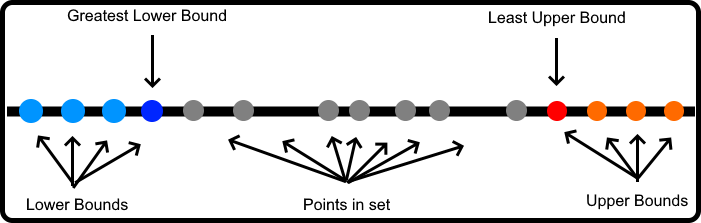
\includegraphics[scale=0.45]{Images/1.2.2.png}
	\end{figure}

	\vspace{0.5cm}





\subsection{ Fields }

	\begin{definition}{Fields Axioms}{14cm}
		\begin{enumerate}[label=(\alph*), leftmargin=0.5cm, itemsep=0.1cm]
			\item Addition Axioms
			
				\begin{itemize}[leftmargin=1cm, itemsep=0.1cm]
					\item If x,y $\in$ F, then x+y $\in$ F
				
					\item x+y = y+x for all x,y $\in$ F
				
					\item (x+y)+z = x+(y+z) for all x,y,z $\in$ F
				
					\item There exists 0 $\in$ F such that 0+x = x for all x $\in$ F
				
					\item For every x $\in$ F, there is -x $\in$ F where x+(-x) = 0
				\end{itemize}

			\item Multiplicative Axioms
			
				\begin{itemize}[leftmargin=1cm, itemsep=0.1cm]
					\item If x,y $\in$ F, then xy $\in$ F
				
					\item yx = xy for all x,y $\in$ F
				
					\item (xy)z = x(yx) for all x,y,z $\in$ F
				
					\item There exists 1 $\not =$ 0 $\in$ F such that
						1x = x for all x $\in$ F
				
					\item If x $\not =$ 0 $\in$ F, there is $\frac{1}{x}$ $\in$ F
						where x($\frac{1}{x}$) = 1
				\end{itemize}

			\item Distributive Law
			
				\hspace{0.5cm}
				x(y+z) = xy + xz hold for all x,y,z $\in$ F
		\end{enumerate}
	\end{definition}

	\vspace{0.5cm}



	\begin{ltheorem}{Consequences of the Field Axioms}{1.5cm}
		\item If x+y = x+z, then y = z
		
			\begin{proof}[14cm]
				y = 0+y = (-x)+x+y = (-x)+x+z = 0+z = z
			\end{proof}
	
		\item If x+y = x, then y = 0

			\begin{proof}[14cm]
				From (a), let z = 0
			\end{proof}
	
		\item If x+y = 0, then y = -x
		
			\begin{proof}[14cm]
				From (a), let z = -x
			\end{proof}
	
		\item -(-x) = x
		
			\begin{proof}[14cm]
				From (c), let x = -x and y = x
			\end{proof}
	
		\item If x $\not =$ 0 and xy = xz, then y = z
			
			\begin{proof}[14cm]
				y = 1y = $\frac{1}{x}$xy = $\frac{1}{x}$xz = 1z = z
			\end{proof}
	
		\item If x $\not =$ 0 and xy = x, then y = 1
		
			\begin{proof}[14cm]
				From (e), let z = 1
			\end{proof}
	
		\item If x $\not =$ 0 and xy = 1, then y = $\frac{1}{x}$
		
			\begin{proof}[14cm]
				From (e), let z = $\frac{1}{x}$
			\end{proof}

			\newpage
	
		\item If x $\not =$ 0, then $\frac{1}{1/x}$ = x
		
			\begin{proof}[14cm]
				From (g), let x = $\frac{1}{x}$ and y = x
			\end{proof}
	
		\item 0x = 0
		
			\begin{proof}[14cm]
				Since 0x + 0x = (0+0)x = 0x = 0x + 0, then 0x = 0
			\end{proof}
	
		\item If x,y $\not =$ 0, then xy $\not =$ 0

			\begin{proof}[14cm]
				Suppose xy = 0, then 1 = $\frac{1}{y}\frac{1}{x}$xy
				= $\frac{1}{y}$$\frac{1}{x}$0 = 0.

				0 = 1 is a contradiction.
			\end{proof}
				
		\item (-x)y = -(xy) = x(-y)
		
			\begin{proof}[14cm]
				xy + (-x)y = (x+(-x))y = 0y = 0.
				Then by part (c), (-x)y = -(xy).

				xy + x(-y) = x(y+(-y)) = x0 = 0.
				Then by part (c), x(-y) = -(xy).
			\end{proof}

		\item (-x)(-y) = xy
		
			\begin{proof}[14cm]
				By part (k), then (-x)(-y) = -[x(-y)] = -[-(xy)].
				By part (d), -[-(xy)] = xy.
			\end{proof}
	\end{ltheorem}

	\vspace{0.5cm}





\subsection{ Ordered Fields }

	\begin{definition}{Ordered Field}{14cm}
		An ordered field F is a field F which is also an ordered set
		for all x,y,z $\in$ F.

		\begin{itemize}[leftmargin=1.5cm, itemsep=0.1cm]
			\item If y $<$ z, then y+x $<$ z+x
		
			\item If x,y $>$ 0, then xy $>$ 0
		\end{itemize}
		
		$ \mathbb{Q} $,$ \mathbb{R} $ are ordered fields,
		but $ \mathbb{C} $ is not an ordered field since i$^2$ = -1 $\not >$ 0.
	\end{definition}
	
	\vspace{0.4cm}



	\begin{ltheorem}{Properties of the Ordered Field}{1.5cm}
		\item If x $>$ 0, then -x $<$ 0 and vice versa
	
			\begin{proof}[14cm]
				-x = -x + 0 $<$ -x + x = 0
			\end{proof}

		\item If x $>$ 0 and y $<$ z, then xy $<$ xz
	
			\begin{proof}[14cm]
				Since z-y $>$ 0, then 0 $<$ x(z-y) = xz - xy
			\end{proof}

		\item If x $ < $ 0 and y $ < $ z, then xy $ > $ xz

			\begin{proof}[14cm]
				Since -x $>$ 0 and z-y $>$ 0, then 0 $<$ -x(z-y) = xy - xz
			\end{proof}
	
		\item If x $\neq$ 0, $x^2 > $ 0

			\begin{proof}[14cm]
				If x $>$ 0 $\Rightarrow$ x$^\text{2}$ = x $\cdot$ x $>$ 0.
				If x $<$ 0 $\Rightarrow$ (-x)$^\text{2}$ = (-x) $\cdot$ (-x)
				= x $\cdot$ x = x$^\text{2}$ $>$ 0
			\end{proof}
	
		\item If 0 $< x < y$, then 0 $< 1/y < 1/x$

			\begin{proof}[14cm]
				($\frac{1}{\text{y}}$)y = 1 $>$ 0 so
				$\frac{1}{\text{y}}$ $>$ 0.				
				Since x $<$ y, then $\frac{1}{\text{y}}$
				= ($\frac{1}{\text{y}}$)($\frac{1}{\text{x}}$)x
				$<$ ($\frac{1}{\text{y}}$)($\frac{1}{\text{x}}$)y
				= $\frac{1}{\text{x}}$.
			\end{proof}
	\end{ltheorem}

	\newpage



	\begin{wtheorem}{$\mathbb{R}$ is an ordered field}{14cm}
		There exists a unique ordered field $\mathbb{R}$ with the
		least upper bound property.

		Also, $\mathbb{Q}$  $\subset$ $\mathbb{R}$ so $\mathbb{Q}$ is
		also an ordered field.
	\end{wtheorem}

	\begin{proof}
		The proof in Day 5 is a construction of $\mathbb{R}$ by defining a
		specific order $<$.
	\end{proof}

	\vspace{0.4cm}



	\begin{ltheorem}{$\mathbb{Q}$  is dense in $\mathbb{R}$}{1.5cm}
		\item {\color{lblue} Archimedean Property}:
			For x,y $\in$ $\mathbb{R}$, if x $>$ 0, there is n $\in$ $ \mathbb{Z} $
			where nx $>$ y.
	
			\begin{proof}[14cm]
				Fix x $>$ 0. Let A = \{ nx: n = 1,2,... \}.
				Suppose there is a y where nx $\leq$ y.

				Then, A is nonempty and bounded from above by y.
				By the least upper bound property of $ \mathbb{R} $,
				$\alpha$ = sup(A) exists in $ \mathbb{R} $ .

				Since x $>$ 0, then -x $<$ 0 so $\alpha - x < \alpha-0 = \alpha$.
				So $\alpha-x$ is not an upper bound of A.
				So there is a mx $\in$ A such that mx $> \alpha-x$.
				Then $\alpha <$ (m+1)x, but (m+1)x $\in$ A
				contradicting $\alpha$ is an upper bound for A.
			\end{proof}

		\item {\color{lblue} $ \mathbb{Q} $  is dense in $ \mathbb{R} $}:
			For x,y $\in$ $\mathbb{R}$, if x $<$ y,
			there is a p $\in$ $ \mathbb{Q} $ where x $<$ p $<$ y.

			\begin{proof}[14cm]
				Since x $<$ y, then y-x $>$ 0. Then by the Archimedean Property,
				there exists n $\in$ Z such that n(y-x) $>$ 1.
				Thus, ny $>$ nx+1 $>$ nx.

				Since there is a smallest m $\in \mathbb{Z_+} $ such that m $>$ nx,
				then m $>$ nx $\geq$ m-1 so nx+1 $\geq$ m $>$ nx.
				Since ny $>$ nx+1 $\geq$ m $>$ nx, then y $>$ m/n $>$ x.
			\end{proof}
	\end{ltheorem}